\begin{frame}
	\frametitle{Motivation}
	\begin{itemize}
		\item The Problem
		\begin{itemize}
			\item Deep Neural Networks
			\begin{itemize}
				\item Requires fixed dimensionality on input and output
			\end{itemize}
		\end{itemize}
		\item The Solution
		\begin{itemize}
			\item Recurrent Neural Network
			\begin{itemize}
				\item Can take a sequence of inputs
				\item Can map a sequence to a fixed size vector
			\end{itemize}
		\end{itemize}
	\end{itemize}


	\note{
		\begin{itemize}
			\item Requires fixed dimensionality on input and output
		\end{itemize}
	}
\end{frame}

\begin{frame}
	\frametitle{The solution}
	\begin{itemize}
		\item Recurrent Neural Network
		\begin{itemize}
			\item Directed cycle
			\item Can take a sequence of inputs
			\item Can map a sequence to a fixed size vector
		\end{itemize}
	\end{itemize}
	\note{
		\begin{itemize}
			\item Holds a cycle
			\item Can take a sequence of inputs
		\end{itemize}
	}
\end{frame}

\begin{frame}
	\frametitle{Recurrent Neural Network}
	\begin{figure}
		\centering
		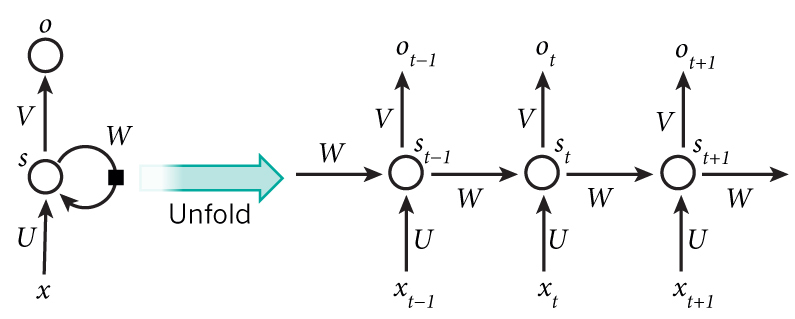
\includegraphics[scale=0.3]{rnn.jpg}
	\end{figure}
\end{frame}

\begin{frame}
	\frametitle{Long short term memory network}
	\begin{figure}
		\centering
		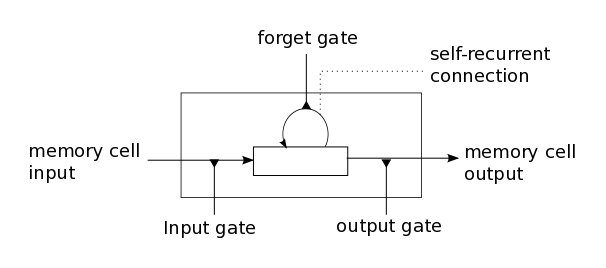
\includegraphics[scale=0.5]{lstm_memorycell.png}
	\end{figure}
\end{frame}

\begin{frame}
	\frametitle{Results}
	\begin{figure}
		\centering
		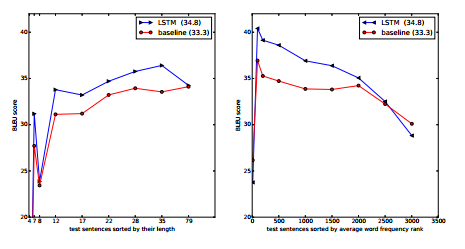
\includegraphics[scale=0.8]{results.png}
	\end{figure}
\end{frame}